%
% File emnlp2020.tex
%
%% Based on the style files for ACL 2020, which were
%% Based on the style files for ACL 2018, NAACL 2018/19, which were
%% Based on the style files for ACL-2015, with some improvements
%%  taken from the NAACL-2016 style
%% Based on the style files for ACL-2014, which were, in turn,
%% based on ACL-2013, ACL-2012, ACL-2011, ACL-2010, ACL-IJCNLP-2009,
%% EACL-2009, IJCNLP-2008...
%% Based on the style files for EACL 2006 by 
%%e.agirre@ehu.es or Sergi.Balari@uab.es
%% and that of ACL 08 by Joakim Nivre and Noah Smith

\documentclass[11pt,a4paper]{article}
\usepackage[hyperref]{emnlp2020}
\usepackage{times}
\usepackage{latexsym}
\usepackage{amsmath,amssymb}
\usepackage{pgfplots}
\usepackage{tikz}
\usepackage{subcaption}
\usepackage{booktabs}
\usepackage{CJKutf8}
\usepackage{makecell}
\usepackage{multirow}
\DeclareUnicodeCharacter{FF08}{fi}
\DeclareUnicodeCharacter{FF09}{fi}
\DeclareUnicodeCharacter{FF0C}{fi}
\renewcommand{\UrlFont}{\ttfamily\small}
\newcommand{\tabincell}[2]{\begin{tabular}{@{}#1@{}}#2\end{tabular}}

% This is not strictly necessary, and may be commented out,
% but it will improve the layout of the manuscript,
% and will typically save some space.
\usepackage{microtype}

%\aclfinalcopy % Uncomment this line for the final submission
%\def\aclpaperid{***} %  Enter the acl Paper ID here

%\setlength\titlebox{5cm}
% You can expand the titlebox if you need extra space
% to show all the authors. Please do not make the titlebox
% smaller than 5cm (the original size); we will check this
% in the camera-ready version and ask you to change it back.
\newcommand{\figref}[1]{Figure \ref{#1}}
\newcommand{\eqnref}[1]{Eq. \ref{#1}}
\newcommand{\tabref}[1]{Table \ref{#1}}
\newcommand{\secref}[1]{Section \ref{#1}}
\newcommand{\algoref}[1]{Algorithm \ref{#1}}
\newcommand\BibTeX{B\textsc{ib}\TeX}
\newcommand{\KZ}[1]{\textcolor{blue}{Kenny: #1}}
\title{A Dataset for Generation of Clarification Questions in Multi-turn Free-style Consultation}

\author{Zengzhen Du, Kenny Q. Zhu, Dan Xie \\
Hubei University of Chinese Medicine / zengzhen@stmail.hbtcm.edu.cn \\
Shanghai Jiao Tong University / kzhu@cs.sjtu.edu.cn \\
Hubei University of Chinese Medicine / dinaxie@hbtcm.edu.cn \\
\texttt{email@domain} \\\And
}

\date{}

\begin{document}
\maketitle
\begin{abstract}
In a consultational dialogue between an expert $E$ and a client $C$, $C$ may fail to
sufficiently describe their cases with $E$. At this point $E$ may need to ask additional
clarification questions to seek further information. In this paper, we propose the following
task for a free-style dialogue system: given a dialogue context, and $E$'s turn to respond,
determine if a clarification question needs to be asked, and if so, 
generate the question automatically. We create a large health consultation dialog dataset
and a labeled test set for this task. We also present some baseline
seq2seq deep neural models that achieve reasonable results.
\end{abstract}

\section{Introduction}

Protein$-$protein interactions (PPIs) are of central importance for the majority of biological functions, such as signal transduction, metabolic pathways, molecular dynamics, and protein networks\cite{Hoffmann.Krallinger.ea:2005}, for they serve as the most fundamental building blocks of the entire interacademic systems of any organisms. Collecting data on pairwise interaction relationships is essential for multiple purpose, including identification of modules with certain functionality\cite{Spirin.Mirny.03}, mapping diseases to dominated genes\cite{Ideker.Sharan.08}, and after all, understanding wholistic metabolic/genetic networks from a system biology perspective.

A lot of databases have been built to store protein and genetic interactions from major model organism species and are available in various standardized formats, such as MINT\cite{Zanzoni.Montecchi-Palazzi.ea:2002}, BIND\cite{Bader.ea:2003}, BIOGRID\cite{DBLP:journals/nar/StarkBRBBT06}, etc. Among those mainstream databases, the data largely rely on voluntary reports by scientists or researchers, besides, comprehensive curation efforts become indispensable for the sake of accuracy. However, the amount of biology-related literatures with respect to protein interactions grows explosively and thus make it either impossible or impractical to manually detect PPI information anymore.

Considering huge amount of PPI information with great wealth hidden in published papers, in recent years, numerous mining techniques have been proposed that aim to extract PPI information automatically from free text, especially machine learning, information retrieval, and natural language processing\cite{DBLP:journals/bib/WinnenburgWPDS08}.These approaches can be roughly categorized into three classes: co$-$occurrence, rule$-$based, and machine learning. 

Co$-$occurrence is the approach with most simplicity and naivete. Just as its name implies, this method intends to find out pairs of proteins that co-occur in the same context. The scope of "same context" ranges from phrase, sentence, paragraph to whole abstract, even document. The underlying assumption is that whenever two proteins are mentioned together by authors, chances are high that there is some kind of relationship between them. However, however, in-context closeness even semantic relation does not necessarily represent actual biological interaction. As a consequence, a large fraction of candidate pairs are mismatched inevitably, causing a high recall but low precision.

The second approach is rule-based extraction, in other words, pattern matching. There are many types of rules, most of them concern natural language processing (NLP). One way is to specify hand-crafted regular expressions before hand, which mostly lean on language usage preference. Besides, by using full or partial (shallow) parsing strategies, more information would be acquired, such as part-of-speech taggers, local dependencies between syntactic components, context-free grammar\cite{DBLP:journals/bioinformatics/TemkinG03}, and full sentence structure. Compared to co$-$occurrence, rule-based approach enjoy better precision but much lower recall. In addition, since the rules are usually derived from training data, that is to say, the improper choice of training data would be significantly lethal, therefore quality of extraction is invariably instable and may not applicable to other data.

The third and most commonly used approach use machine learning techniques, in this case, the task to extract protein$-$protein interactions turns out to be a binary classification problem. Each protein pairs are represented along with a set of features, which is associated with their context, then a well$-$defined classifier gives the answer whether the candidate protein pairs is classified to be qualified PPI. (TO BE FURTHER FILLED!!!)

In this paper, we introduce a general bootstrapping framework for Protein$-$protein interaction extraction from natural text.Our method differs from most of the previous works in three aspects:

(1)The extraction process is driven by only tiny fraction of training data, which are regarded as seed data. In each round, it would derive reliable patterns automatically from seed data, then extract more positive PPI pairs consequently, what's more, the seed data would be augmented by the newly extracted results with high confidence.

(2)multiple graph kernel. 

(3)various evaluation.




\section{Problem Definition}
\label{sec:problem}

In this section we formally define the problem of short title extraction.
A char is a single Chinese or English character.
A segmented word (or term) $x$ is a sequence of several chars such as 
``Nike'' or ``牛仔裤''(jean).
A product title, denoted as $X$, is a sequence of words $\{x_1, x_2, ..., x_n\}$.
Let $Y$ be a sequence of labels $\{y_1, y_2, ..., y_n\}$ over $X$, where $y_i \in \{0, 1\}$.
The corresponding short title is a subsequence of $X$, denoted as $S = \{x_i\}$, 
where $y_i = 1$ and $|S| \le n$.

%we are interesting in obtaining a short title which can represent the most important information about the product.

We regard short title extraction task as a sequence classification problem.
Each word is sequentially visited in the original product title order
and a binary decision is made.
We do this by scoring each word $x_i$ within $X$ and predicting a label $y_i \in \{0, 1\}$, 
indicating whether the word should or should not be included in the short title $S$.
As we apply supervised training, the objective is to maximize the likelihood of all word labels
$Y=\{y_1,y_2,...,y_n\}$, given the input product title $X$ and model parameters $\theta$:
\begin{equation}
\label{eqn:problem}
\log{p(Y|X,\theta)}=\sum_{i=1}^{n}{\log{p(y_i|X,\theta)}}.
\end{equation}

%Our problem is different from Sequece Labelling problem, as ...

%In a more restrictive scenario, the number of words $m$ in the short title is strictly limited, where $m$ is some fixed number and $m \le \sum_{i=1}^{n} len(x_i)$. $len(x_i)$ is the number of words (chars) in term $x_i$.


\subsection{Dataset}
\label{sec:data}
To train and evaluate our approach of detecting false rumors, a labeled
data set is needed.
We collect a set of known false rumors from Sina community management center \cite{website:Manage},
which deals with reporting
of issues including various misinformation which we regard as
certified false rumors.
% consists of all kinds of fields, so the diversity of rumors is guaranteed.
There are 11466 reported false rumors between 2012/05/28 and 2014/04/11.
%in the result publication category at that time excluding the those without links for the original message webpages.
%Above rumor data are captured directly from Sina Weibo's mobile website.
Since a rumor must have sufficient circulation, we only keep those false
rumors that have at least 100 reposts, which leaves us with 2601 false rumors
up to 2014/04/11.
%and all their reposting information by the time of being captured excluding abnormal original message links.
%Some previous works \cite{yang2012automatic} also made use of
%Sina Weibo's official acount to collect false rumors.
%But at that time, Sina Weibo had not constructed the community management
%and there was an only official false rumor busting account in
%Sina Weibo posting some identified misinformation to public.
%One problem is that the false rumor reports posted by the account
%had no links to the original messages so they needed to
%construct queries manually to find out the original messages.
Sina Weibo API provides interfaces to capture the information of
original messages as well as their repost messages.
From Sina Weibo API, we captured the post time, post client
and content of 2601 false rumors along with all their reposts.

In the real world, the number of false rumors on Sina Weibo
is much smaller than the number of normal messages (1 out of 9 or less).
Thus a ``dummy'' classifier that rules all messages as normal messages
will achieve a very high accuracy (above 90\%) on real-world data.
To avoid this problem, we construct a data set with roughly equal number of
false rumors and normal messages. Most studies in the past also use
data sets which are either 50-50 split
\cite{castillo2011information,jin2013epidemiological}
or close to that \cite{yang2012automatic,qazvinian2011rumor}.
Thus, we randomly select 5000 other Weibo original messages
which are not proved to be false as well as their reposts
using the Sina Weibo API. Then, we manually filtered out messages with fewer than 100 reposts as well as false rumors to form a set of 2536 normal messages.
%To make non-rumors be in accord with rumors, we also only select the tweets that have 100 reposts at least here. The profiles of users involved are included in the data captured from API. Afterwards, we labeled 2844 pieces of non-rumors from them manually.
Each message or repost contains links to the author profile
information such as age, gender, number of followers and friends,
and can be crawled using the Weibo API.
%
%Sina Weibo provides API to capture a user's information but the speed is too slow because of frequency restriction. So we capture the original poster's information through Sina Weibo API and the other users' information directly from their homepages on Sine Weibo's mobile website.
%

At the end of this phase, our labeled data set 
\footnote{The labeled data set of the original messages (without reposts)
is available at \url{http://adapt.seiee.sjtu.edu.cn/~kzhu/rumor/}.}
consists of 2601 false rumors, 2536 normal messages
and with 4 million distinct users involved in these messages. Of these
500 false rumors and 500 other messages (called small data set) are used for
SVM parameter tuning while
the rest (called big data set) are used for end-to-end cross validation.

\section{Approach}
%We first present our methods for testing short circuits in
%models, then modify some of these methods to create
%training data to reverse the short circuit problem
%and enhance the robustness of the models.
% 
%\subsection{Proxy Test for Short Circuit}
%We propose two types of approaches that can be used as proxy test for short circuits.
%One is through inspecting attention maps in
%the models under a white-box setting.
%The other is to generate new test cases by applying different operations on correct choices under a black-box setting.
%
%
%\subsubsection*{White-box Attention Weights~(AW)}
%One intuitive way to detect if an attention-based model is 
%exploiting short circuits is to visualize its attention map. 
%Given a well-trained model and a correctly answered MCQ  in the 
%form of \textit{[CLS] premise [SEP] choice [SEP]}, 
%where \textit{[CLS]} and \textit{[SEP]} are model-dependent 
%delimiters and \textit{choice} refers to the correct choice, 
%we first tokenize the input, feed the token sequence into the model, 
%and extract the attention map of all attention heads from the 
%last encoder layer.
%
%The attention maps are visualized through off-the-shelf tool~\cite{vig-2019-multiscale}
%into user-friendly demo as shown in \figref{fig:att-goodex}. 
%Human annotators are then asked to determine whether there exists 
%strong attention connections from the correct choice to the premise. 
%We consider the MCQ is solved without short-circuiting only if 
%over half of the annotators label it as having strong attention 
%connections. 
%
%Though accurate, such manual annotation is cost-prohibitive to be 
%scaled to larger tests. To remedy this issue, we propose 
%a rule-based procedure to automatically detect the short circuit 
%behavior of a model on MCQ. Specifically, we aggregate the 
%attention maps into one individual map by max-pooling over all 
%attention heads. Then we check if there exists at least one 
%attention score between token in the choice and token in the premise 
%higher than threshold $t_1$ or at least two higher than threshold 
%$t_2$, excluding special tokens like comma and period. 
%We consider that the model not short-circuiting on this MCQ if 
%neither of the two conditions is met. In practice, the 
%threshold $t_1$ and $t_2$ are tuned so as to maximally simulate 
%human annotation. The pseudo-code is shown in Algorithm \ref{AW}.
%
In this section, we first present our methods for testing short circuits in models, and then modify some of these methods to create training data to address the short circuit problem and enhance model robustness.

\subsection{Proxy Test for Short Circuit}
Since no existing method can definitively prove if a model is short-circuiting on a question, we propose two types of approaches that serve as proxy tests for short circuits. These approaches reveal the effects of model short-circuiting, though they can't directly prove the short-circuit itself, similar to dark matter. One approach involves inspecting attention maps in models under a white-box setting, while the other generates new test cases by applying different operations on correct choices under a black-box setting.

\subsubsection*{White-box Attention Weights~(AW)}

One intuitive way to detect if an attention-based model is exploiting short circuits is to visualize its attention map. Given a well-trained model and a correctly answered MCQ in the form of \textit{[CLS] premise [SEP] choice [SEP]}, where \textit{[CLS]} and \textit{[SEP]} are model-dependent delimiters and \textit{choice} refers to the correct choice, we first tokenize the input, feed the token sequence into the model, and extract the attention map of all attention heads from the last encoder layer.

The attention maps are visualized through an off-the-shelf tool~\cite{vig-2019-multiscale} into a user-friendly demo, as shown in \figref{fig:att-goodex}. Human annotators are then asked to determine whether there exists strong attention connections from the correct choice to the premise. We consider the MCQ to be solved without short-circuiting only if over half of the annotators label it as having strong attention connections.

Although accurate, such manual annotation is cost-prohibitive to be scaled to larger tests. To remedy this issue, we propose a rule-based procedure to automatically detect the short circuit behavior of a model on MCQ. Specifically, we aggregate the attention maps into one individual map by max-pooling over all attention heads. Then we check if there exists at least one attention score between a token in the choice and a token in the premise higher than threshold $t_1$, or at least two higher than threshold $t_2$, excluding special tokens like comma and period. We consider the model to not be short-circuiting on this MCQ if neither of the two conditions is met. In practice, the thresholds $t_1$ and $t_2$ are tuned to maximally simulate human annotation. The pseudo-code is shown in Algorithm \ref{AW}.


\begin{algorithm}
\small
	\caption{Attention Weight Thresholding}
	\label{AW}
\hspace*{0.02in} {\bf Input:} 
premise $P$, correct choice $C$, model $M$,  threshold $t_1$ and $t_2$. \\
\hspace*{0.02in} {\bf Output:}
binary 0/1 label $L$.
	\begin{algorithmic}[1]
		\State initialize counters $c_1$ and $c_2$ to 0.
		\State tokenize the formatted input as sequence of tokens $S$.
		\State feed $S$ into $M$ and extract the last layer's attention maps $Attn_{all}$.
		\State aggregate $Attn_{all}$ into $Attn_{max}$ by max-pooling over all attention heads.
		\For{$w_1$ in $C$}
		\For{$w_2$ in $P$}
		\If{$Attn_{max}(w_1, w_2)> t_1$}
				$c_1$ += 1
		\EndIf
		\If{$Attn_{max}(w_1, w_2) > t_2$}
				$c_2$ += 1
		\EndIf
		\EndFor
		\EndFor
		\State output 1 if $c_1>0$ or $c_2\geq 2$ and 0 otherwise.
	\end{algorithmic}
\end{algorithm}

\subsubsection*{Black-box Choice Operator}
\label{sec:proxy}
While attention-based testing methods can detect short circuits within the encoder directly, they don't directly detect short circuits in the end-to-end MCQ model, which also includes a linear layer above the attention-based pretrained language model. Additionally, these methods are limited to a family of models with inherent attention mechanisms.

A more desirable approach is an automatic end-to-end black-box test that is model-independent. In black-box testing, if a model correctly answers an MCQ, we slightly modify the MCQ by applying a certain``operation'' on the original correct choice to produce another wrong choice. The newly generated MCQ must share the same correct choice as the original question. By observing the model's response to the second MCQ, we can infer whether the model short-circuits on the original MCQ.If the model still selects the correct choice, then we consider it to have passed the test and not short-circuited on the original MCQ. The challenge now is how to construct the new wrong choice by implementing the operation in various ways.

In this paper, we consider the operations listed in \tabref{table:proxyop}. Some of the operations were mentioned in previous literature, while others are proposed here (marked with *).
The first line in each cell describes the operation, and the next two lines provide an example of constructing a false choice from a choice in the original question. An operation may either preserve (p) the truth value (\crosssymbol $\rightarrow$ \crosssymbol) or change (c) the truth value of the choice (\checksymbol $\rightarrow$ \crosssymbol).

\begin{table}[th]
        \centering
        \scriptsize
        \begin{tabular}{l|l}
                \toprule
                \textbf{Oper.} &\textbf{Description and Example}\\
                \hline
                \multirow{3}{*}{Neg+} & Add negation (c) \\
                & \textit{They called the police to come to my house. \checksymbol} \\
                & \textit{They {\color{olive}{didn't}}  called the police to come to my house. \crosssymbol} \\
                \hline
                \multirow{3}{*}{Neg-} &Remove negation (c) \\
                & \textit{Ben {\color{olive} never} starts working out. \checksymbol} \\
                & \textit{Ben starts working out. \crosssymbol}\\
                \hline

                \multirow{3}{*}{NER} &Randomly replace person names (c)\\
                 & \textit{A big wave knocked {\color{olive} Mary} down . \checksymbol} \\
                & \textit{A big wave knocked {\color{olive} Kia} down . \crosssymbol} \\
                \hline
                \multirow{3}{*}{PR*} & Switch pronoun by gender or quantity (c)\\
        &\textit{{\color{olive} She} had a great time .\checksymbol} \\
        &\textit{{\color{olive} He} had a great time . \crosssymbol} \\
                \hline
                \multirow{3}{*}{PI*} &Instantiate pronoun by randome person (c) \\
        &\textit{{\color{olive} They} gave Tom a new latte with less ice . \checksymbol}\\
        &\textit{{\color{olive} Nathanael} gave Tom a new latte with less ice . \crosssymbol}\\
                \bottomrule
%               \hline
                \multirow{3}{*}{Adv} &Add adverbs for emphasis (c) \\
                &\textit{The ocean was a calm as a bathtub .\crosssymbol} \\
                &\textit{{\color{olive} In fact} the ocean was a calm as a bathtub .\crosssymbol} \\
                \hline
               \multirow{3}{*}{CO*} & Crossover: Swap the true choices between two questions (p)\\ 
	&\textit{\color{olive}Josh got sick . \checksymbol} \\
	&\textit{\color{olive}{She had a great time .\crosssymbol}}  \\
\hline
                \multirow{3}{*}{Syn} &Replace adj/adv with synonym (p) \\
                &\textit{Dawn felt {\color{olive} happy} about getting away with it . \crosssymbol} \\
                &\textit{Dawn felt {\color{olive} glad} about getting away with it . \crosssymbol} \\

		\bottomrule
               \multirow{3}{*}{MT*} & Mutate: Swap two consecutive words (c) \\
		& \textit{Deb said yes {\color{olive} to} {\color{olive} Tim} 's marriage proposal. \crosssymbol} \\
		& \textit{Deb said yes {\color{olive} Tim} {\color{olive} to} 's marriage proposal .\crosssymbol} \\
               \hline
\multirow{3}{*}{Voice} &Swap subject and object (c) \\
        & \textit{{\color{olive}{Kara}} asked {\color{olive}{the neighbors}}  not to litter in their yard . \checksymbol} \\
        &\textit{{\color{olive}{the neighbors}} asked  {\color{olive}{Kara}}  not to litter in their yard . \crosssymbol}\\
                \bottomrule
        \end{tabular}
        \caption{A number of operations considered for proxy testing. 
First line in each cell describes the operation, the next two lines
give an example of how to construct a false choice from a choice of
the original question. An operation may either 
preserve (p) the truth value (\checksymbol $\rightarrow$ \checksymbol, \crosssymbol $\rightarrow$ \crosssymbol) or change (c) the truth value of
the choice (\checksymbol $\rightarrow$ \crosssymbol).  }
        \label{table:proxyop}
\end{table}

Inspired by boundary testing in software engineering, we can classify these operations into three equivalent classes (three vertical sections in \tabref{table:proxyop}), depending on the nature of the \textit{false} choice constructed:
\begin{enumerate}
\item The syntax and semantics are correct, and the \textit{false} choice appears similar to the \textit{true} choice.
\item The syntax and semantics are correct, and the \textit{false} choice appears distinct from the \textit{true} choice.
\item Either syntax or semantics is incorrect.
\end{enumerate}

The last class is not suitable for testing short circuits because the model may answer the proxy question correctly by eliminating the false choice due to errors in it, not by considering the premise.

We focus on perturbations on negation~\cite{checklist2020acl}, NER~\cite{checklist2020acl}, and pronouns in the first class and adverbial~\cite{wsp2020acl}, crossover, and synonym~\cite{checklist2020acl,wsp2020acl} in the second class.

While most of the operations are self-explanatory, the \textit{crossover} operation is unique and deserves special attention. Inspired by molecular biology, for each MCQ in the dataset that the model answers correctly, we substitute the original false choice with the true choice from another randomly sampled MCQ. The substituted choice remains false in the proxy question. The operation can be visually explained in \figref{fig:cross}.

\begin{figure}[th]
\centering
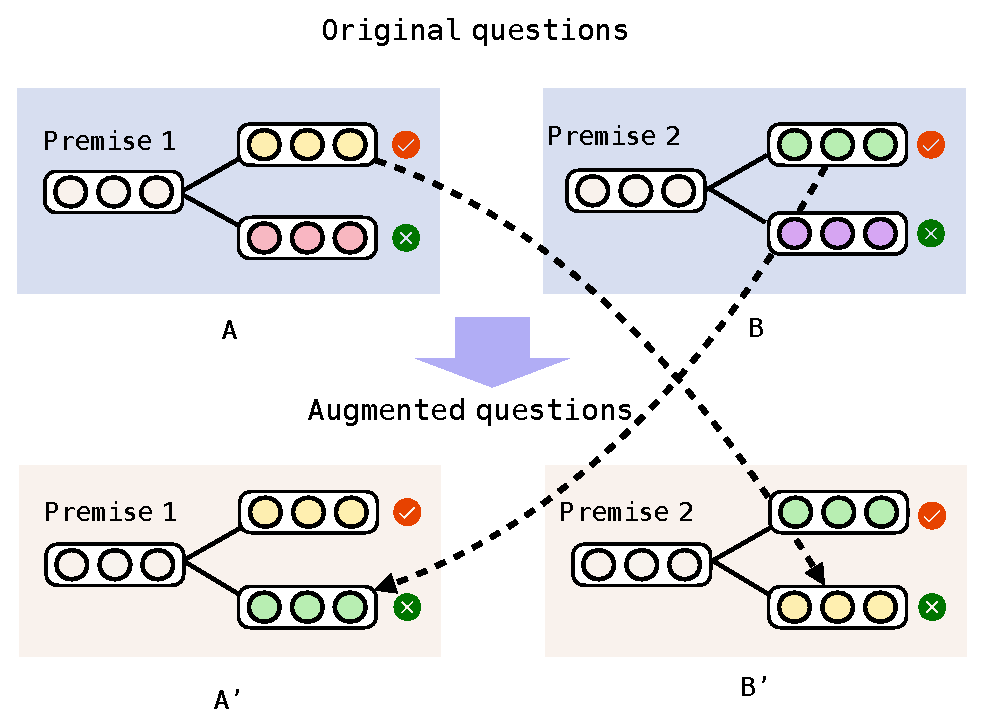
\includegraphics[width=\columnwidth]{figure/cross.eps}
\caption{The Crossover Operation: the true choice of both questions
are used to replace the false choices of these questions to create
two new proxy questions.}
\label{fig:cross}
\end{figure}

Compared to all other operations in classes 1 and 2, the crossover provides a proxy question that is most different from the original one but easier from a human perspective. This is because the two choices may be quite unrelated. If the model does not handle it correctly, it may be more indicative of a short circuit. As a result, the crossover is potentially a better short circuit test than others.

Another advantage of the crossover operation is that we can generate multiple false choices for an original question at a low cost, allowing us to test each original question more thoroughly. In contrast, most other operations cannot produce an adequate number of different variants of the original choice.

In summary, the proposed black-box choice operator provides a more generalizable and model-independent method for detecting short circuits in MCQ models. By applying various operations to create proxy questions, we can assess the model's performance and robustness more accurately, contributing to the development of better and more reliable models in the future.

\subsection{Improving Model Robustness by Data Augmentation}

If a model is shown to short-circuit by the proxy tests, its performance may decline, especially when applied to out-of-domain test data. To make models more robust, one natural thought is to generate more data to encourage models to focus on the relation between the premise and choices. While the operations used to generate proxy tests can also be utilized for data augmentation, not all of them are scalable or able to generate enough data for training.

The two operations that can generate a substantial amount of data are crossover and mutation. These operations can be applied to the training data to enhance the model's robustness.

\subsubsection*{Crossover for Data Augmentation}

Crossover is a good option for data augmentation because the two choices were originally true answers in their respective questions and presumably carry spurious features if the model was short-circuiting. By incorporating crossover into the training data, the model is forced to consider the premise in order to determine which choice is better.

\subsubsection*{Mutation for Data Augmentation}

Mutation has two flavors: (1) swap the words only in the true choice; (2) swap the words both in the true and the false choice. Compared to crossover, mutation has the potential to be more effective at improving model robustness. It not only forces the model to look into the premise due to its two very similar choices (same set of tokens), but also makes the model more sensitive to fine differences in word orders and enhances the model's prior grammatical knowledge.

\subsubsection*{Differentiating between Proxy Test and Data Augmentation}

It is essential to differentiate between the use of crossover and mutation operations in proxy tests and data augmentation. In proxy tests, these operations are used to modify the test data to assess the model's short-circuiting behavior. In contrast, when applied for data augmentation, the same operations work on the training data to enhance the model's robustness and generalization capabilities.

In conclusion, data augmentation through crossover and mutation operations can contribute to improving model robustness by encouraging models to focus on the relationship between the premise and choices. By incorporating these operations into the training data, models are forced to consider the premise and become more sensitive to the fine differences in word orders, leading to better performance and reliability in real-world applications.


\section{Experiments}
We first expound our pruning setting
and provide evidences for its ability to identify relation-specific subnetworks in PLM.
Then we experiment on several commonsense-intensive scenarios to seek 
good practices for using these subnetworks.

\subsection{Disentangling PLMs into Relation-specific Subnetworks}
\label{sec:LAMA}
\begin{table}[!h]
	\centering
	\small
	\begin{tabular}{l|cc}
		\toprule
		\textbf{Data Split} & \textbf{\# Rels} & \textbf{\# Prompts} \\
		\midrule
		Train  & 16 &  20,841\\
		Validation   & 16 &  5,955\\
		Test   & 16 &  2,978\\
		\bottomrule
	\end{tabular}
	\caption{Statistics of C-LAMA.}
	\label{table:conceptnet}
\end{table}
\noindent
\textbf{Dataset.}~~We use the ConceptNet~\citep{speer-havasi-2012-representing} subset of LAMA benchmark as supervision, denoted as C-LAMA.
C-LAMA contains commonsense facts from the English part of ConceptNet that has
single-token objects covering 16 relations. These facts are extracted from Open Mind Common Sense~(OMCS) and will be used as cloze-prompts for pruning. We construct the train/valildation/test splits with a ratio of 7:2:1. Detailed statistics is listed in \tabref{table:conceptnet}. Precision P@K is used to evaluate the prompt filling performance. For a given $\mathcal{LM}$, we save subnetworks that achieve highest micro-averaged P@1 on the validation set and report the micro-averaged P@K on the test set.
%\KZ{What confuses me a bit is that the pruning matrices are trained on C-LAMA, and then testedb-[]
%also on C-LAMA, then what makes it a weak-supervision? How do you determine the train-test split
%on C-LAMA?}


\noindent
\textbf{Models.}~~For the choices of $\mathcal{LM}$, we consider the 6-layer \textsc{DistilBERT-base}~\citep{DBLP:journals/corr/abs-1910-01108}, 12-layer \textsc{BERT-base}, 12-layer \textsc{RoBERTa-base}~\citep{DBLP:journals/corr/abs-1907-11692}. We also include the more recent 12-layer \textsc{MPNet-base}~\citep{song2020mpnet} model. All models are implemented with HuggingFace's transformers~\citep{DBLP:journals/corr/abs-1910-03771} library. 

\noindent
\textbf{Setup.}~~The prior distribution $\phi(\cdot)$ is a Gaussian $\mathcal{N}(\mu, 1)$ where $\mu$ is the mean controlling initial sparsity of pruned model~(e.g., $\mu=0$ indicates $50\%$ initial sparsity).
We set $l_t$ to be the top layer of a given model 
and choose $l_b$ from $\{3,4\}$ for \textsc{DistilBERT}, $\{6,7,8,9\}$ for \textsc{BERT}, \textsc{RoBERTa}, 
and \textsc{MPNet}. The temperature $\tau$ is fixed as $0.1$. The threshold $t$ is fixed as $0.5$. 
We use Adam~\citep{kingma2014method} with a batch size of $32$ and a linear warm-up scheduler 
with $0.1$ warm-up ratio for training the mask up to $6$ epochs. 
The learning rate is fixed as $3\times 10^{-4}$. All experiments are conducted on a GTX 1080 Ti GPU with 11G RAM.
% \KZ{Table 1 indicates
%that the sparcity of all three models under deterministic pruning is around 50\%, which is the same
%as the initial sparcity. This means nothing is done?? Also this sparcity issue seems not mentioned in the method section?
%How we do control the sparcity? Why do we need to control it? Does it have anything to do with the accuracy of
%the subnet thus obtained?} 


%\KZ{The organization of the following experiments seems a bit
%arbitrary. Maybe first give an overview of what experiments will be done next
%and their logical connection?}
\begin{figure}[t!]
	\centering
	\scalebox{1.0}{\includegraphics[width=1.0\columnwidth]{figure/both.pdf}}
	\caption{Ablation on the pruning masks~(left) and effect of initial sparsity and pruned layers~(right).} \label{fig:both}
\end{figure}
\noindent
\textbf{Factors impacting performance.}~~~To investigate how $\mu$ and $l_b$ influence the  performance, we perform a preliminary experiment by applying deterministic pruning on \textsc{BERT-base} with $l_b$ in $\{6,7,8,9\}$ and initial sparsity in $\{50\%,54\%,58\%,62\%\}$.  \figref{fig:both}~(right) shows that (i)~increasing the number of pruned layers helps distill more knowledge. (ii)~larger initial sparsity is more likely to prune away weights important to certain knowledge and cannot be recovered in the later training process. In general, we find an initial sparsity around $50\%$ yields decent performance both in probing and downstream applications. We adopt this setting in the remainder of this paper unless state otherwise.
\begin{table*}[t!]
	\centering
	\scriptsize
	\begin{tabular}{l|ccc|c|c|c}
		\toprule
		\textbf{Model} & \textbf{P@1~(\%)} & \textbf{P@2~(\%)} & \textbf{P@3~(\%)} & \textbf{Sparsity}  & $\bm{l_b-l_t}$ & \textbf{\# Param.}\\
		\midrule
		\textsc{DistilBERT} w/o pruning& 11.4 &16.6  &19.9  & 0\% & - & 66M\\
		\textsc{DistilBERT} w/ stochastic pruning & 14.8 &21.5 &26.3 & $\sim$30\% & 4-6 &66M \\
		\textsc{DistilBERT} w/ deterministic pruning & 44.1 &52.9 &57.6 & $\sim$50\% & 4-6 &56M \\
		\midrule
		\textsc{BERT} w/o pruning& 12.9 & 18.4  & 21.8 & 0\% & -  &110M\\
		\textsc{BERT} w/ stochastic pruning & 17.2 & 25.1  & 29.6  & $\sim$30\% & 7-12 & 110M\\
		\textsc{BERT} w/ deterministic pruning & 57.6 & 63.8  & 67.2  & $\sim$50\% & 7-12 & 88M\\
		\midrule
		\textsc{RoBERTa} w/o pruning& 15.4 & 21.2  & 24.6 & 0\% & - &125M  \\
		\textsc{RoBERTa} w/ stochastic pruning &16.6  &22.2   &25.8   & $\sim$30\% & 7-12 & 125M\\
		\textsc{RoBERTa} w/ deterministic pruning &38.3  &42.8   &44.6   & $\sim$50\% & 7-12 &100M \\
		\midrule
		\textsc{MPNet} w/o pruning& 14.8  &20.7   &24.0 & 0\%  & - & 110M\\
		\textsc{MPNet} w/ stochastic pruning &19.8  &27.9   &33.2  & $\sim$30\% & 7-12  & 110M\\
		\textsc{MPNet} w/ deterministic pruning &62.7  &68.7   &71.4  & $\sim$50\% & 7-12 &88M \\
		%		\midrule
		%		\textsc{BERT-base-finetuned-CoNLL03} w/o pruning&0.0  &0.0   &0.0 & 0\% & -  & 110M\\
		%		\textsc{BERT-base-finetuned-CoNLL03} w/ deterministic pruning & 27.1 & 37.7  & 43.1 & $\sim$50\% & 7-12 & 88M\\
		%		\midrule
		%		\textsc{BERT-base-finetuned-SQuAD} w/o pruning&0.0  &0.0   &0.0  & 0\% & - & 110M\\
		%		\textsc{BERT-base-finetuned-SQuAD} w/ deterministic pruning & 22.5 & 32.4  & 37.5 & $\sim$50\% & 7-12 & 88M\\
		\bottomrule
	\end{tabular}
	\caption{Relational knowledge probing results on C-LAMA. We relegate the 
		complete results to Appendix.}
	\label{table:rank}
\end{table*}

\noindent
\textbf{Disentanglement between subnetworks.}~~Properly disentangled subnetworks are expected to perform poorly on relations other than their associated ones. We verify this by instantiating the pruning mask upon \textsc{BERT-base} with a set of mismatched masks.
Specifically, we corrupt the correspondence of relation between masks and prompts by shifting the order of masks 15 times, as there are 16 relations in total. Then we calculate the micro-averaged P@K for each shift and average the results. As shown in \figref{fig:both}~(left), If we apply the mismatched masks from other relations, the P@1  score significantly drops to $4.8$, even inferior to the original model. It shows that the representation spaces for different commonsense relations modeled by these subnetworks are highly disentangled and  exhibits remarkably distinct geometry.

We also examine the non-triviality of subnetworks by initializing the masks with a Bernoulli distribution $B(0.5)$ and averaging the results from 5 different random seeds.
If we apply such random masks with sparsity comparable to learned ones, the P@1 drops drastically to $0.4$. This notable gap proves that the effective subnetworks cannot be trivially identified through random weights sampling.

\noindent
\textbf{Comparision with original models.}~~We present the full results of all models in \tabref{table:rank}. Among all models without pruning, \textsc{RoBERTa} achieves the highest P@1 score of $15.4$ while \textsc{DistilBERT} gets the lowest $11.4$. It indicates that while PLMs are shown to be helpful for downstream learning, they cannot accurately complete cloze-like prompts that require commonsense relation knowledge. This observation also coincides with previous finding~\citep{inductivemlm} that the uniform masking adopted by PLMs is biased towards extracting statistical and syntactic dependencies. 
Comparing the results for each pair of original and subnetworks, we consistently observe a surprisingly significant increase~(37.0 on average), especially for deterministically pruned ones. This large performance gap provides unique new evidence of sparse latent relational knowledge structures in PLMs, which are weakened by pretrained weights that are \textit{reserved} for more general-purpose use. 

We also observe that the deterministic pruning excels by a huge margin 
across all models, which implies that representation subspaces for relational knowledge deviate largely from the original language representation space. Another advantage of deterministic pruning in memory 
footprint is that only sets of 1-bit masks rather than 32-bits float parameters 
need to be saved for solving multiple tasks. For the above reasons, 
we focus our analysis on and use \textsf{pruned} to denote deterministically 
pruned PLMs in the rest of this paper. 
%\KZ{Why deterministic ones are so much better than stochastic ones?
%THis is a bit counter-intuitive.}
%\KZ{To show that you have successfully disentangled the network into 16 subnets, each corresponds to a relation
%in C-LAMA, maybe you should also show that a subnet for $r_i$ works not so well for relation $r_j$ where
%$i \ne j$, but works very well for $r_i$?  Later in Fig 2 (left) you showed this result. But does it come a bit too
%late? You have only showed the latter in Table 1. But of course, $r_i$ and
%$r_j$ need to be semantically distinct in the first place.}



%\KZ{What's the diff between this subsubsection and the previous one about ``to what extent we can
%disentangle? It seems that to show the extent u can disengle u need to show that
%the subnets are very different? But that's doesn't seem to be so important.
%Maybe u can consider merging these two subsubsections.}


%\begin{figure}[t]
%	\centering
%	\scalebox{1.0}{\includegraphics[width=1.0\columnwidth]{figure/vertical.png}}
%	\caption{Effect of initial sparsity and pruned layers.} \label{fig:vertical}
%\end{figure}

%\KZ{Only now you talk about the significance of the
%initial sparcity. This comes a bit too late. Reorg the presentation
%so that readers are not left in puzzle at all.}


\noindent
\textbf{Visualization of attention weights and representations.}~~To explain 
how the subnetworks accommodate more accurate commonsense knowledge despite 
having far fewer weights than the full-scale models, we randomly 
sample several prompts that the subnetworks correctly answered but 
the full-scale model~(\textsc{BERT-base}) failed to and 
visualize the attention patterns in the last layer.
\begin{table*}[t!]
	\centering
	\scriptsize
	\begin{tabular}{l|cccc|cccc}
		\toprule
		\multirow{2}{*}{\textbf{Model}} & \multicolumn{4}{c|}{\textbf{Development Set}} &\multicolumn{4}{c}{\textbf{Test Set}}  \\
		
		&MRR~(\%)   &P@1~(\%)  &P@2~(\%)  &P@3~(\%)  &MRR~(\%)   &P@1~(\%)  &P@2~(\%)  &P@3~(\%)  \\
		\cline{1-9}
		\textbf{\textit{Supervised}} & & & & & & & &\\
		\cline{1-9}
		\textsc{DistMult}~\citep{yang2015embedding} &8.5   &4.2  &6.6  &8.3  &10.5   &5.4  &8.4  &10.9  \\
		\textsc{ComplEx}~\citep{complex} &10.7   &6.5  &9.0  &11.0  &13.6   &8.2  &12.4  &15.7  \\
		\textsc{ConvE}~\citep{DBLP:journals/corr/DettmersMSR17} &18.9   &11.5  &16.6  &19.0  &21.9   &13.5  &18.9  &24.0  \\
		\textsc{TuckER}~\citep{DBLP:journals/corr/abs-1901-09590} &17.3   &10.9  &14.8  &18.8  &21.6   &14.0  &20.4  &24.0  \\
		\textsc{ConvTransE}~\citep{shang2019end-to-end} &19.8   &13.2  &17.8  &21.3  &24.0   &\textbf{15.6}  &21.9  &\underline{26.5}  \\
		\textsc{SACN}~\citep{shang2019end-to-end} &21.2   &13.2  &19.8  &23.2  &\textbf{24.2} &14.4  &\underline{22.1}  &\textbf{28.0}  \\
%		\textsc{InteractE}~\citep{DBLP:journals/corr/abs-1911-00219} &20.5   &12.2  &18.3  &22.2  &\textbf{25.0}   &\underline{15.0}  &\textbf{23.6}  &\textbf{29.0}  \\
		\midrule
		\textbf{\textit{Unsupervised}} & & & & & & & &\\
		\cline{1-9}
		\textsc{DistilBERT} &9.0 &3.1 &6.9 &10.3 &10.8 &5.8 &9.6 &11.2 \\
		\textsc{BERT} &12.4 &7.2 &10.0 &13.7 &14.3 &8.3 &13.7 &16.6 \\
		\textsc{RoBERTa} &8.3 &4.2 &6.0 &7.1 &9.4 &5.1 &7.1 &9.3 \\
		\textsc{MPNet} &11.7 &7.2 &9.4 &11.1 &11.1 &6.0 &9.9 &11.7 \\
		\midrule
		\textsc{DistilBERT}~(pruned) &\textbf{24.1} &\textbf{15.8} &\textbf{24.1} &\underline{26.4} &\underline{23.4} &\underline{14.8} &\textbf{22.2} &\underline{26.5} \\
		\textsc{BERT}~(pruned) &\underline{23.7} &\underline{15.5} &\underline{22.1} &\textbf{27.0} &22.8 &14.3 &20.9 &26.0 \\
		\textsc{RoBERTa}~(pruned) &9.0 &4.9 &7.1 &8.9 &9.5 &6.1 &7.6 &11.4 \\
		\textsc{MPNet}~(pruned) &22.1 &12.9 &21.2 &25.5 &20.0 &11.4 &18.8 &22.9 \\
		\bottomrule
	\end{tabular}
	\caption{Link prediction results. Best results are marked with \textbf{bold} font and second best with \underline{underline}.}
	\label{table:linkprediction}
\end{table*}
\begin{figure}[th]
	\centering
	\scalebox{1.0}{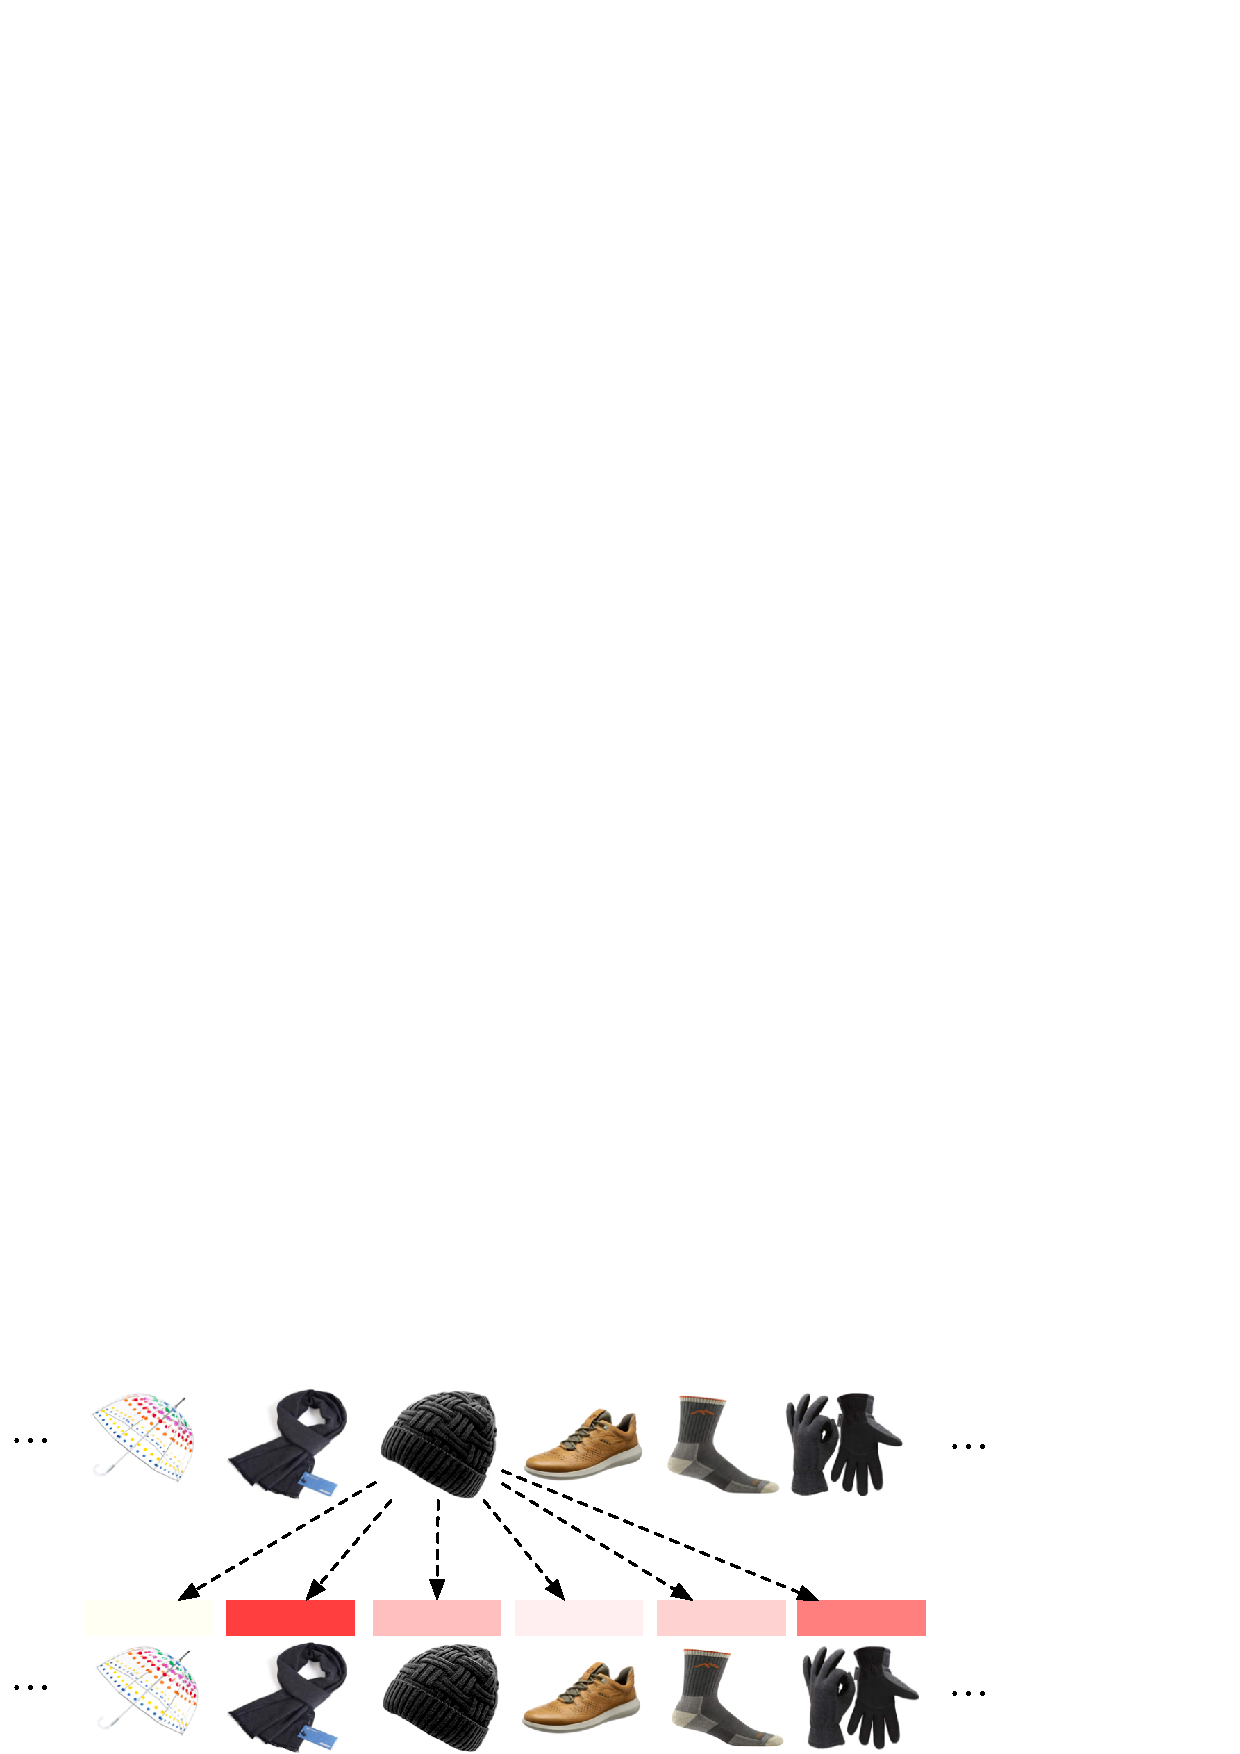
\includegraphics[width=1.0\columnwidth]{figure/attention.pdf}}
	\caption{Attention weight visualization. \textit{AtLocation} is required for prompt in the left column and \textit{PartOf} is required for prompt in the right column.} \label{fig:attention}
\end{figure}
Specifically, we focus on the attention weights between [MASK] token and 
other tokens in the prompt. A first glance of change of attention pattern 
is given in \figref{fig:LAMA} and we show more examples of other ConcetpNet 
relations in \figref{fig:attention}. We observe that while the original 
pretrained model tends to attend to special tokens like period and [SEP], 
the subnetwork successfully grasps the relevant concepts~(i.e., apple, 
worms, and basement) in the prompt hence produces the right object. 
We also use t-SNE~\citep{vanDerMaaten2008} to visualize the last layer's 
representation of [CLS] for each prompt. From \figref{fig:tsne}, the 
representations computed by original pretrained model are hardly separable as 
different types of knowledge are mixed together. In contrast, the pruned 
subnetwork can extract meaningful and disentangled representations for 
different commonsense relations.

\begin{figure}[th]
	\centering
	\scalebox{1.0}{\includegraphics[width=1.0\columnwidth]{figure/tsne_compare.pdf}}
	\caption{t-SNE visualization of [CLS]'s representation from original~(left) and pruned~(right) \textsc{BERT-base}.} \label{fig:tsne}
\end{figure}


\subsection{Commonsense Knowledge Base Completion~(CKBC)}
\label{sec:ckbc}
We evaluate the utility of identified relation-specific subnetworks on CKBC in an unsupervised manner. Specifically, we use the ConceptNet-100K benchmark provided by \citet{Li2016}. To ensure a fair evaluation, 
we manually create a subset of ConceptNet-100K 
consisting of triples with single-token subject/object. We also ensure that its dev/test set has \textbf{no overlap} with C-LAMA.
Each relation is associated with a sentence template~(provided in 
Appendix)~\citep{Kwon2019} of which the wording is distinct from 
those in C-LAMA. We acknowledge that these sentence templates might be suboptimal for certain relations, but prompt optimization is 
out of the scope of this paper. The resulting dataset contains 
$17,891$ training instances, $349$ development instances, 
and $446$ test instances.

\textbf{Link prediction.}~~We first formulate CKBC as a link prediction task 
and compare subnetworks~(i.e., $\mathcal{LM}_{\theta_r}$ 
is queried to predict missing link for instance of relation $r$) as well as original PLMs
against strong supervised KB completion mothods. 


\tabref{table:linkprediction} shows the results. Most of the supervised 
models outperform full-scale PLMs by a large margin, which suggests the 
inefficacy of directly using PLMs to perform link prediction. However, 
the subnetworks identified by our pruning procedure can
acquire performance on par with or better than state-of-the-art 
supervised models. Surprisingly, the pruned \textsc{DistilBERT} get the 
highest MRR, outperforming other larger and more advanced PLMs. 
\textsc{RoBERTa} struggles to predict correct objects, perhaps due to 
its larger vocabulary size compared to WordPiece~($50,265$ vs $30,522$) 
and less lexicon overlap~($53\%$ vs $59\%$) with the dataset.

%\KZ{It seems that our method (pruned models) don't work so well in the
%test set, compared to dev set. The scores for the same model between dev set and
%test set are also quite diff. Can you explain in this para?}

\textbf{Triple classification}~~We can also formulate CKBC as a triple classification task. Following ~\citet{Feldman2020}, we use estimated point-wise mutual information~(PMI) computed by pretrained language model as a surrogate of a triple's validity. An expectation-maximization-based Gaussian mixture clustering method is used and instances in the cluster with higher mean PMI are labeled as valid. 
\begin{table}[t]
	\centering
	\scriptsize
	\begin{tabular}{l|c}
		\toprule
		\textbf{Model} &  \textbf{F1 Score}\\
		\midrule
		\textsc{DistilBERT} & 74.1\\
		\textsc{DistilBERT}~(pruned) & \textbf{76.3}\\
		\midrule
		\textsc{BERT} & 73.7\\
		\textsc{BERT}~(pruned) & \textbf{76.7}\\
		\midrule
		\textsc{RoBERTa} &74.8 \\
		\textsc{RoBERTa}~(pruned) & \textbf{76.9}\\
		\midrule
		\textsc{MPNet} &76.5 \\
		\textsc{MPNet}~(pruned) & \textbf{78.0}\\
		\bottomrule
	\end{tabular}
	\caption{Triple classification on ConceptNet-100K.}
	\label{table:tripleclassification}
\end{table}
In our preliminary experiments, we found that the model pruned by the mask 
of a single relation might not be robust for PMI estimation and generally 
performed inferior to the intact model. 
In the same spirit as model ensembling, we then perform grid search over 
combinations of multiple knowledge, which is similar to what we did 
in zero-shot commonsense reasoning. For all four PLMs considered in 
\tabref{table:tripleclassification}, we observe that there exists one 
or multiple knowledge combinations delivering F1 score higher than the 
original models. 
%\KZ{Why is the difference between pruned and unpruned models
%not so big compared to link prediction?}

\textbf{Triple extraction.}~~We then investigate the ability of specialized 
subnetworks to extract novel commonsense knowledge triples absent 
from the dataset. We randomly sample 100 triples from the test set of 
ConceptNet-100K and for each sample use top-$K$ predictions from 
pruned \textsc{DistilBERT-base} as candidate objects. 
Three human annotators are asked to first determine the correctness of 
each candidate object and further determine their novelty~(i.e., not present 
in any of train/validation/test set) if deemed to be correct. 
The Fleiss Kappa inter-annotator agreement $\kappa$ is 0.66/0.65 
for precision and novelty, respectively.
\begin{figure}[t]
	\centering
	\scalebox{0.7}{\includegraphics[width=1.0\columnwidth]{figure/precision_novelty_2.pdf}}
	\caption{Precision-novelty curve with varied $K$.} \label{fig:extraction}
\end{figure}
\figref{fig:extraction} shows the change of precision-novelty with varied $K$. We observe a clear trade-off between the validity and novelty of triples extracted by the pruned model. As expected, a large $K$ inevitably makes noisy predictions but is more likely to extract unseen knowledge. For the purpose of knowledge enrichment, one might choose a large $K$ to ensure a desirable recall. We list the obtained novel triples in the Appendix D due to space limits.






\subsection{Commonsense Reasoning~(CSR)}
\label{sec:csr}
After identifying sparse subnetworks within PLMs that specialize in different commonsense knowledge, we now evaluate their generalization ability in the context of commonsense reasoning.
%One desirable outcome of our pruning procedure is the transformation from language representation to knowledge representation. We test if such subnetworks generalize in the context of commonsense reasoning.

\textbf{Many-shot learning.}~~We experiment with \textsc{BERT-base} and its deterministically pruned version using supervised fine-tuning on $7$ datasets: RTE~\citep{CambridgeJournals:6906264}, COPA~\citep{roemmele_choice_2011}, CommonsenseQA~\citep{talmor-etal-2019-commonsenseqa}, SWAG~\citep{zellers-etal-2018-swag}, HellaSWAG~\citep{DBLP:journals/corr/abs-1905-07830},   aNLI~\citep{DBLP:journals/corr/abs-1908-05739} and CosmosQA~\citep{huang-etal-2019-cosmos}. For each task, we identify the commonsense knowledge it might requires with a simple heuristic. Specifically, we obtain the five most frequent relations~(measured by how many times subject and object of certain relation appear in the context or answer) for each task and perform grid search over the combinations of these relationns. Then we take the union of masks for each relation and apply the resultant mask to the BERT as initialization for finetuning.
We repeat the training three times with different random seeds for each task. 
The  choice of mask combination for each task can be found in Appendix B.

The results in \tabref{table:finetuning} shows that, when initialized with proper weights, the model can be better fine-tuned on downstream commonsense reasoning tasks via more useful \textit{prior} knowledge. We further analyze the change of performance under the low-resource regime on COPA dataset. \figref{fig:copa} shows that the pruned \textsc{BERT} exhibits a notable advantage when training data is extremely scarce. As more training data is seen, the benefit of the pruned 
model becomes less prominent, i.e., $p>0.05$.
\begin{table}[t!]
	\centering
	\scriptsize
	\begin{tabular}{l|cc|c}
		\toprule
		\textbf{Task} & \textbf{Original} & \textbf{Pruned} &$p$-value \\
		\midrule
		RTE & 69.2$\pm${\scriptsize 2.3} & 69.8$\pm${\scriptsize2.0}& 0.12\\

		COPA & 62.4$\pm${\scriptsize 5.0} & 63.0$\pm${\scriptsize 4.7} &0.33  \\

		CommonsenseQA & 53.1$\pm${\scriptsize 0.6} & 54.1$\pm${\scriptsize 0.7} &0.08\\

		SWAG & 73.9$\pm${\scriptsize 0.3} & 74.2$\pm${\scriptsize 0.1} &0.09\\
		HellaSWAG & 38.9$\pm${\scriptsize 0.4} & 39.1$\pm${\scriptsize 0.5}&0.32  \\
		aNLI &63.7$\pm${\scriptsize 0.4} &64.0$\pm${\scriptsize 0.4}  &0.19\\
		CosmosQA &61.3$\pm${\scriptsize 1.0} &61.8$\pm${\scriptsize 0.2} &0.26\\
		\bottomrule
	\end{tabular}
	\caption{Finetuning results of \textsc{BERT} for CSR.}
	\label{table:finetuning}
\end{table}
\begin{figure}[t]
	\centering
	\scalebox{0.75}{\includegraphics[width=1.0\columnwidth]{figure/copa.pdf}}
	\caption{Finetuning result of \textsc{BERT} on COPA with varying portion of data.} \label{fig:copa}
\end{figure}
\begin{table*}[t!]
	\centering
	\scriptsize
	\begin{tabular}{l|cccccccc|c}
		\toprule
		\textbf{Model} &COPA-Tra. &COPA-Val. &CSQA &CA &WSC  &SM &ARCT1 &ARCT2 &Avg. \\
		\midrule
		\textsc{DistilBERT} &58.3 &60.0 &29.6 &84.6 &53.3  &71.6 &48.6 &50.4  &57.0  \\
		\textsc{DistilBERT}~(pruned) &\textbf{61.5} &\textbf{69.0} &\textbf{31.5} &\textbf{89.6} &\textbf{56.9}  &\textbf{72.1} &\textbf{53.4} &\textbf{51.6} & \textbf{60.7} \\
		\midrule
		\textsc{BERT} &60.2 &54.0 &26.5 &89.0 &57.3  &69.7 &46.8 &50.3 &56.7 \\
		\textsc{BERT}~(pruned) &\textbf{63.0} &\textbf{64.0} &\textbf{28.5} &\textbf{91.8} &\textbf{59.0}  &\textbf{71.7} &\textbf{50.0} &\textbf{52.0}  & \textbf{60.0}\\
		\midrule
		\textsc{RoBERTa} &60.7 &59.0 &39.9 &90.1 &61.8  &73.1 &48.6 &53.1 &60.7 \\
		\textsc{RoBERTa}~(pruned) &\textbf{65.3} &\textbf{72.0} &\textbf{40.4} &\textbf{93.4} &\textbf{62.9}  &\textbf{74.4} &\textbf{53.2} &\textbf{55.1} &\textbf{64.6}\\
		\midrule
		\textsc{MPNet} &66.5 &69.0 &40.0 &94.5 &64.3&75.8  &52.9 &56.7 &64.9  \\
		\textsc{MPNet}~(pruned) &\textbf{71.0} &\textbf{74.0} &\textbf{41.7} &\textbf{97.3} &\textbf{66.4}  &\textbf{77.5} &\textbf{56.1} &\textbf{57.7}  & \textbf{67.7}\\
		\bottomrule
	\end{tabular}
	\caption{Zero-shot results of accuracy~(\%) on commonsense reasoning tasks. Better results of each pair is in \textbf{bold}.}
	\label{table:zeroshot}
\end{table*}



\textbf{Zero-shot learning.}~~We next assess the ability of specialized 
subnetworks to perform zero-shot commonsense reasoning, a setting where 
the knowledge relied on to complete the task is solely determined by the model 
parameters. Here we focus on the following multiple-choice datasets: training set of COPA~(COPA-Tra.), validation set of COPA~(COPA-Val.), CommonsneseQA, Conjunction 
Acceptability~(CA)~\citep{Zhou2019}, 
Winograd Schema Challenge~(WSC)~\citep{levesque_winograd_2012}, 
SenseMaking~(SM)~\citep{wang-etal-2019-make}, 
ARCT1~\citep{habernal-etal-2018-argument} and 
ARCT2~\citep{DBLP:journals/corr/abs-1907-07355}. Each sample in the above datasets can be formulated as $\{[CLS]~context~[SEP]~choice_i ~[SEP]\}_{i=1}^{N}$, where $i$ is the subscript and $N$ is the number of choices. We compute the plausibility score of each choice using MLM head. Choice with the highest plausibility score is chosen as the answer. 

Since multiple types of knowledge are typically required for effectively 
reasoning over concepts, for each task, we perform grid search over 
combinations of $3$-$4$ different commonsense knowledge out of 
the $16$ total types and reported the best accuracy in \tabref{table:zeroshot}. 
We put the best combination for each model on each task in Appendix B
for space constraints. By combining multiple commonsense knowledge useful for the task, 
we show that the pruned models can actually surpass their full-scale 
version in all tasks considered in our experiments. 
The most likely explanation is that knowledge irrelevant to the specific task 
in the original models hurt the in-domain zero-shot reasoning capability. 
It also manifests that the most important reasoning skills vary from 
task to task.

\section{Related Work}
This section surveys previous works on question generation and tree encoding
respectively.

Text question generation has attracted the attention 
after the work of ~\citeauthor{du2017learning}~\shortcite{du2017learning}, who uses deep seq2seq model 
to generate questions from a raw text paragraph. 
Before that, text question generation relied heavily on hand-craft 
question patterns~\cite{HeilmanS10,LabutovBV15,MostowC09} which is time and 
labor consuming. 

However, this pure seq2seq model is not focused and 
has no control over part in the paragraph to generate question. 
~\citeauthor{zhou2017neural}~\shortcite{zhou2017neural} proposed to encode 
key phrase information using binary indicators to generate 
key-aware questions and they assumes the answer to be key phrase. 
Considering key phrase (answer) is unavailable in reality, 
~\citeauthor{SubramanianWYT17}~\shortcite{SubramanianWYT17} applied 
a two-stage approach. First, key phrases are extracted by 
pointer network~\cite{ptrnet}. Second, 
key phrases are encoded in the same way as 
Zhou et al. With the intuition that questions could be asked in many ways, 
~\citeauthor{Yao2018vae}~\shortcite{Yao2018vae} used conditional-VAE to 
increase the diversity of questions. More recently, models with 
auxiliary feature information~\cite{HarrisonW18} helped improve 
the question quality. Structure question generation aims at 
converting structured data such as triples in knowledge graph to questions. 
~\citeauthor{SerbanGGACCB16}~\shortcite{SerbanGGACCB16} proposed a model to generate factoid questions from knowledge base triples.  None of the above work
considered using parse tree structures to aid question generation process,
which is the focus of this paper.

Sequential RNN model takes sentence as a sequence of words, 
ignoring the syntactic information. In order to utilize
such syntactic information with sequential information, 
~\citeauthor{tai2015improved}~\shortcite{tai2015improved} proposed Tree-LSTM to 
encode the binary parse tree recursively in a bottom-up fashion to 
classify sentiment. In text generation task, 
\citeauthor{eriguchi2016tree}~\shortcite{eriguchi2016tree} 
proposed a tree-to-sequence model with attention mechanism to do 
machine translation and 
~\citeauthor{liang2018automatic}~\shortcite{liang2018automatic} proposed a 
tree-to-sequence model which could handle arbitrary trees, 
to do code comment generation. Our work is inspired by these previous
attempts and we are first to adapt structure encoded neural models to
textual question generations.
\section{Conclusion}
\label{sec:conclude}
In this work,
we propose a new data creation method to generate
 a semi-structured synthetic training data for 
opinion summarization,
which is known for lacking training data.
\cut{We showed that by extracting an aspect-opinion pairs and 
implicit sentences from multiple reviews
first and then synthesizing them into semi-structured data, we achieve
better performance on opinion summarization.}
%\KZ{It is critical to show in your experiments that the proposed
%synthetic data is better than other possible alternatives.}, 
We also designed an aspect-guided model with opinion-aspect pair encoder and implicit sentence encoder.
The results showed that
the proposed model can make full use of semi-structured data
and generate high-quality summaries.



	
\bibliography{emnlp2020}
\bibliographystyle{acl_natbib}
%\appendix
	
\end{document}
